\section{Motivation \& Objective}

\begin{frame}{}

\vspace*{1cm}

{\huge{\textbf{Motivation \& Objective}}}

\end{frame}


\begin{frame}[t]{\huge{{\textbf{Motivation \& Objective}}}}

\begin{columns}
    \begin{column}[t]{0.5\textwidth}

        \uncover<1->{
          \begin{itemize}
              \item<2-> \only<2>{\textbf{The missing baryon problem}} \only<3->{The missing baryon problem}
              \item<3-> \only<3>{\textbf{WHIM} : $\text{T} \sim 10^5-10^7$ K \\ \hspace*{13mm} $\text{n}_\text{H} \sim 10^{-6}-10^{-4} \ \text{cm}^{-3}$} \only<4->{WHIM : $\text{T} \sim 10^5-10^7$ K \\ \hspace*{13mm} $\text{n}_\text{H} \sim 10^{-6}-10^{-4} \ \text{cm}^{-3}$}
              \item<4-> \only<4>{\textbf{BLAs : Way to probe WHIM}} \only<5->{BLAs : Way to probe WHIM} 
              \item<5-> \only<5>{\textbf{Survey of BLAs}} \only<6->{Survey of BLAs} 
              \item<6-> \only<6>{\textbf{Baryon content in BLAs} ($\Omega_\mathbf{b}(\textbf{BLA})$)} 
        \end{itemize}
        }
        
    \end{column}      

    \begin{column}[t]{0.5\textwidth}

        \uncover<2>{
          \begin{figure}[!htbp]
            \centering
            \includegraphics<2>[width=5cm]{Figures/Baryon_distribution.png} %
            \vspace*{-1mm}
            \caption{Baryon budget at $z \sim 0$.\\ Shull et al. (2012)}
          \end{figure}}

          \uncover<3>{
          \begin{figure}[!htbp]
            \centering
            \vspace*{-20.75mm}
            \includegraphics<3>[width=5cm]{Figures/Baryon_distribution.png} %
            \vspace*{-1mm}
            \caption*{\textcolor{caption-blue}{Figure 1:} Baryon budget at $z \sim 0$.\\ Shull et al. (2012)}
          \end{figure}}

        \uncover<4->{
          \begin{figure}[!htbp]
              \centering
              \vspace*{-20mm}
              \includegraphics<4->[width=6cm]{Figures/BLA-individual.png}
              \vspace*{-1mm}
              \caption{A BLA towards the LOS of quasar H 1821+643.\\ Philipp Richter (2005)}
          \end{figure}}

    \end{column}

    \begin{tikzpicture}[remember picture, overlay,use page relative coordinates]
  
      \uncover<2->{\node at (0.20,0.17) {\footnotesize{Ref. : Shull et al. (2012)}} ;}
      \uncover<4->{\node at (0.235,0.13) {\footnotesize{Lehner et al. (2007)}} ;}
      
    \end{tikzpicture}

\end{columns}

\end{frame}


% \begin{frame}[noframenumbering]{\huge{{\textbf{Motivation \& Objective}}}}

% \begin{columns}
%     \begin{column}{0.5\textwidth} 
%         \vspace{-10.5mm}
%         \uncover<1->{
%           \begin{itemize}
%               \item The missing baryon problem
%               \item \textbf{BLAs : Way to probe WHIM}
%               \item[]    
%               \item[]    
%         \end{itemize}
%         }
%     \end{column}      

%     \begin{column}{0.5\textwidth}
%         \uncover<1->{\begin{figure}[!htbp]
%           \centering
%           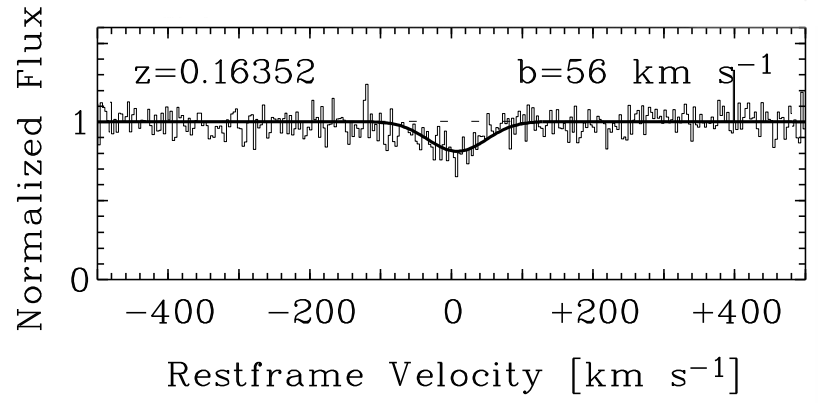
\includegraphics[width=6cm]{Figures/BLA-individual.png}
%           \vspace*{-1mm}
%           \caption{A BLA towards the LOS of quasar H 1821+643.\\ Philipp Richter (2005)}
%         \end{figure}}
%     \end{column}

% \end{columns}


% \begin{tikzpicture}[remember picture, overlay,use page relative coordinates]
  
%   \uncover<1->{\node at (0.20,0.17) {\footnotesize{Ref. : Shull et al. (2012)}} ;
%   \node at (0.235,0.13) {\footnotesize{Lehner et al. (2007)}} ;}
  
% \end{tikzpicture}

% \end{frame}


% \begin{frame}[noframenumbering]{\huge{{\textbf{Motivation \& Objective}}}}

% \begin{columns}
%     \begin{column}{0.5\textwidth} 
%         \vspace{-14.74mm}
%         \uncover<1->{
%           \begin{itemize}
%               \item The missing baryon problem
%               \item BLAs : Way to probe WHIM
%               \item \textbf{Survey of BLAs}
%               \item[]   
%         \end{itemize}
%         }
%     \end{column}      

%     \begin{column}{0.5\textwidth}
%         \uncover<1->{\begin{figure}[!htbp]
%             \centering
%             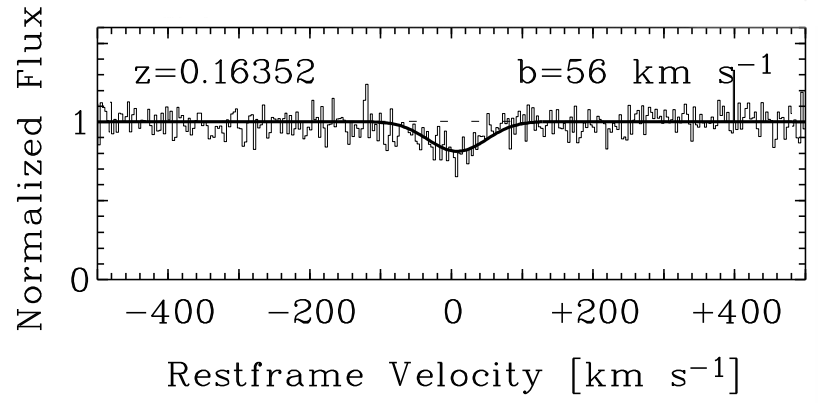
\includegraphics[width=6cm]{Figures/BLA-individual.png}
%             \vspace*{-1mm}
%             \caption{A BLA towards the LOS of quasar H 1821+643.\\ Philipp Richter (2005)}
%           \end{figure}}
%     \end{column}

% \end{columns}

% \begin{tikzpicture}[remember picture, overlay,use page relative coordinates]
  
%   \uncover<1->{\node at (0.20,0.17) {\footnotesize{Ref. : Shull et al. (2012)}} ;
%   \node at (0.235,0.13) {\footnotesize{Lehner et al. (2007)}} ;}
  
% \end{tikzpicture}

% \end{frame}


% \begin{frame}[noframenumbering]{\huge{{\textbf{Motivation \& Objective}}}}

% \begin{columns}
%     \begin{column}{0.5\textwidth} 
%         \vspace{-12.56mm}
%         \uncover<1->{
%           \begin{itemize}
%               \item The missing baryon problem
%               \item BLAs : Way to probe WHIM
%               \item Survey of BLAs
%               \item \textbf{Baryon content of BLAs} 
%         \end{itemize}
%         }
%     \end{column}      

%     \begin{column}{0.5\textwidth}
%         \uncover<1->{\begin{figure}[!htbp]
%             \centering
%             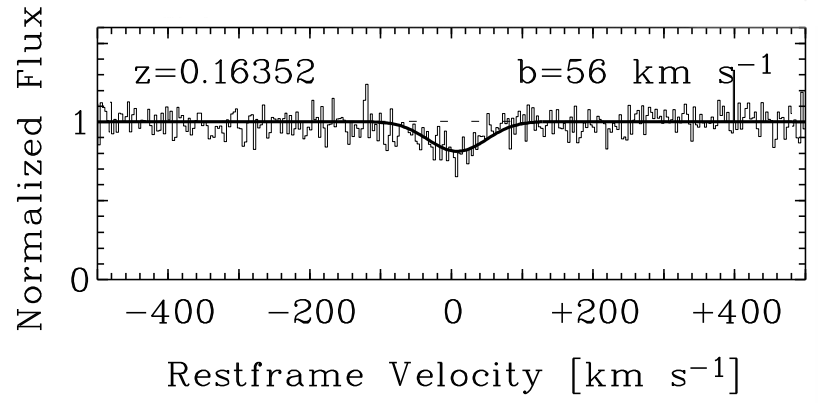
\includegraphics[width=6cm]{Figures/BLA-individual.png}
%             \vspace*{-1mm}
%             \caption{A BLA towards the LOS of quasar H 1821+643.\\ Philipp Richter (2005)}
%           \end{figure}}
%     \end{column}

% \end{columns}

% \begin{tikzpicture}[remember picture, overlay,use page relative coordinates]
  
%   \uncover<1->{\node at (0.20,0.17) {\footnotesize{Ref. : Shull et al. (2012)}} ;
%   \node at (0.235,0.13) {\footnotesize{Lehner et al. (2007)}} ;}
  
% \end{tikzpicture}

% \end{frame}